\documentclass [11 pt, twoside] {article}


\def \jtitle {Lie groups}
\def \jlecturer {Richard Borcherds}
\def \jterm {}
\def \jauthor {Jack DeSerrano}


\usepackage [course] {jack}

\title {Lie groups}
\author {Jack DeSerrano}

\begin {document}

\maketitle

These notes are based on Richard Borcherds's YouTube series on Lie groups.\footnote{See \url{https://www.youtube.com/playlist?list=PL8yHsr3EFj53RWBkiHKoOsTw-dGHAoJ-h}.}

\begin {figure}
	\begin {center}
		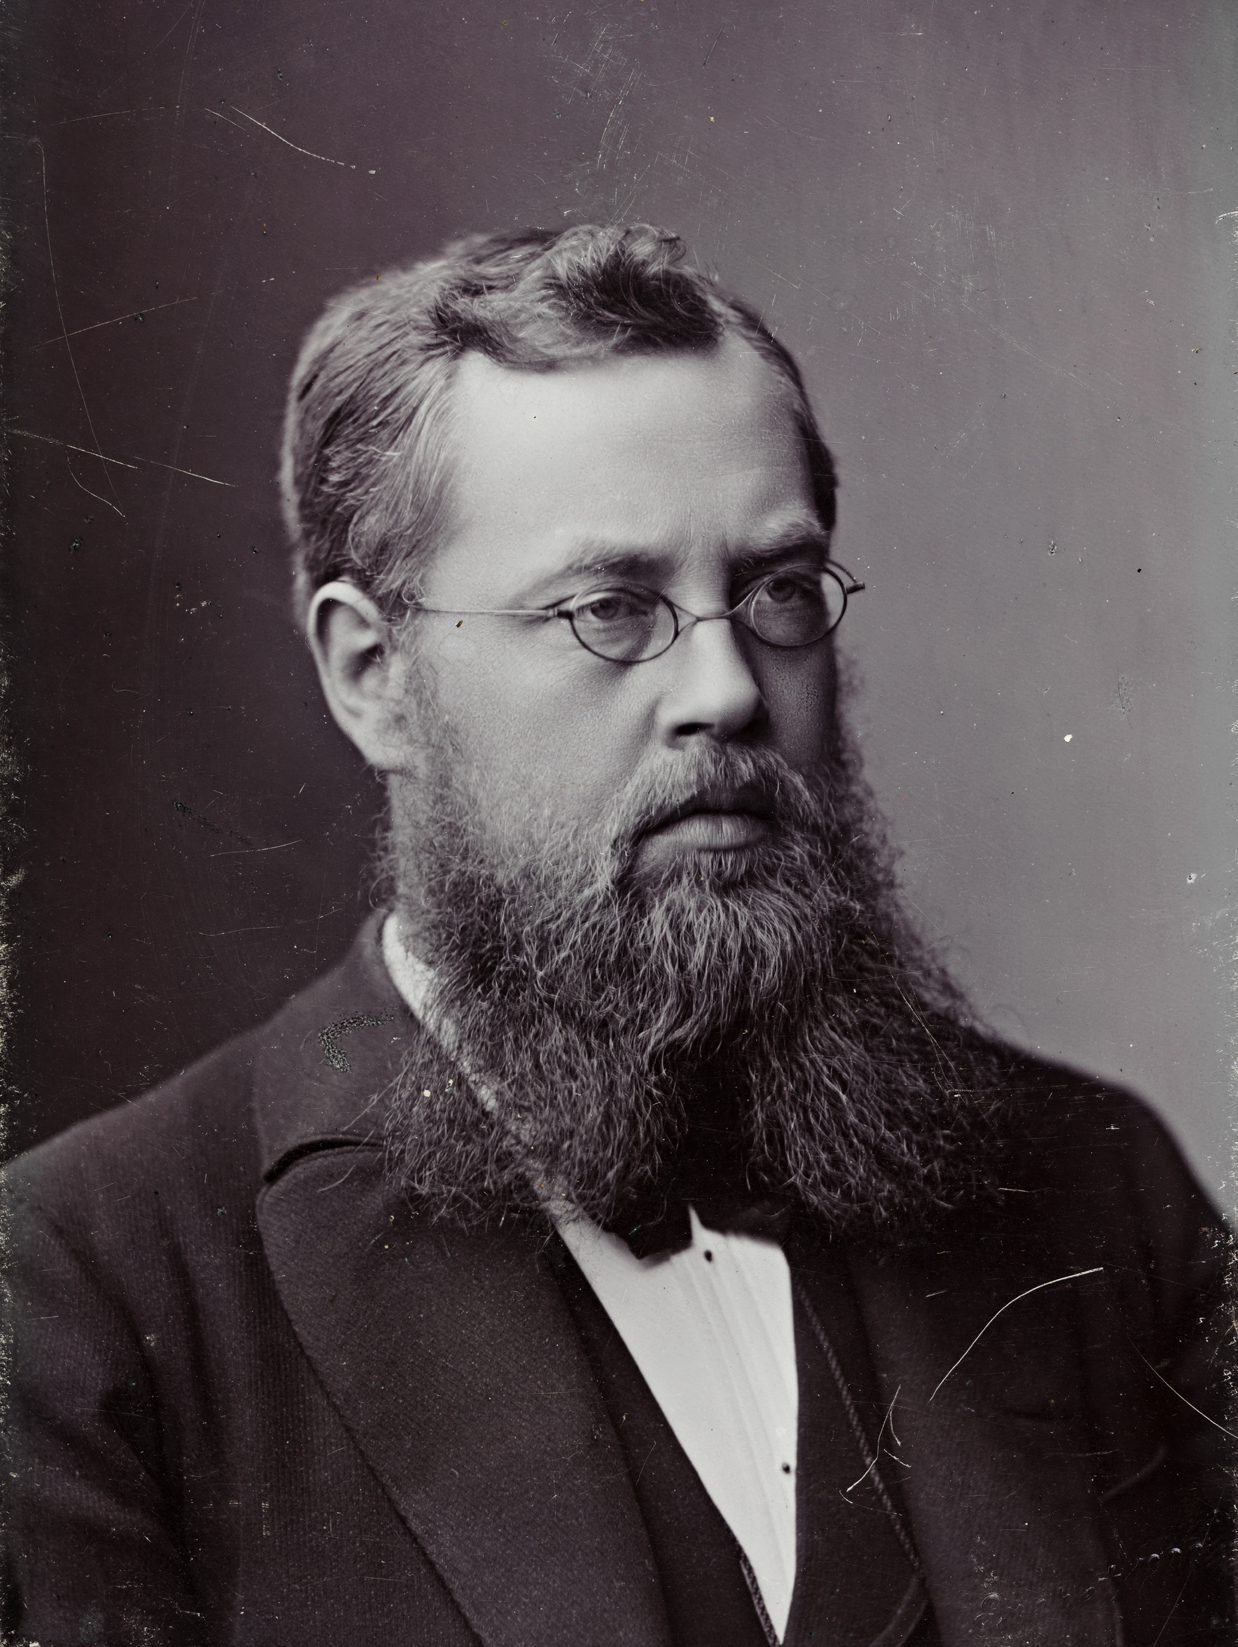
\includegraphics [scale = 0.33] {images/lie}
		\caption {Sophus Lie.}
	\end {center}
\end {figure}
% https://upload.wikimedia.org/wikipedia/commons/a/a3/Portrett_av_Sophus_Lie.jpg
% https://www.flickr.com/photos/48220291@N04/8447487830

\newpage

\iffalse
	\hypersetup {linkcolor = black}
	\tableofcontents
	\hypersetup {linkcolor = Red}
\fi

\section {Introduction}
First thing's first:
\begin{align*}
	\textrm{Lie} = \textrm{li\textlengthmark}
\end{align*}

A \defn{Lie group}\index{Lie group} is a group and a manifold, so, locally, it looks like $\mathbf{R}^{n}$. The number $n$ is the \defn{dimension}\index{dimension of a Lie group} of the Lie group.

The group $\GL_{n}(\mathbf{R})$ is a Lie group of dimension $n^{2}$: It is an open subset of the space of $n\times n$ matrices. 

Lie groups of dimension $0$ are, essentially, the same as discrete groups.
The classification of discrete groups is completely hopeless.
However, any Lie group $G$ has a connected component $G\sub{con}$ that is a normal subgroup of $G$.\footnote{This group is also a Lie group.}
The quotient $G\sub{disc} = G/G\sub{con}$ is $0$-dimensional.
Thus, one can split a Lie group into a discrete part and a connected part. One can, more or less, classify the connected Lie groups.

\begin{example}[ ]\label{}\text{}
Take $G:= \mathbf{R}^{*}$. 
Then, $G\sub{con} = \mathbf{R}_{>0}$ is the connected part and $G\sub{disc} = \{+,-\}$ is the discrete part.
\end{example}

The groups $\mathbf{R}$ under addition, $\mathbf{R}^{*}$ under multiplication, and $S^{1}\subset \mathbf{C}^{*}$ are $1$-dimensional Lie groups.
There are group homomorphisms
\[
\begin{tikzcd}
	\exp:\mathbf{R}\ar[r] & \mathbf{R}^{*}
\end{tikzcd}
\]
and
\[
\begin{tikzcd}
	\mathbf{R}^{*}\ar[r] & S^{1} : z\ar[r,mapsto] & e^{2\pi i z}.
\end{tikzcd}
\]
The second homomorphism is a \defn{local isomorphism}\index{local isomorphism}.
Any connected $1$-dimensional Lie group is isomorphic to $\mathbf{R}$ under addition or $S^{1}$ under multiplication.

Clearly, $\mathbf{R}^{1}\times \mathbf{R}^{1} = \mathbf{R}^{2}$, $\mathbf{R}^{1}\times S^{1}$, and $S^{1}\times S^{1}$ are $2$-dimensional Lie groups. 
Each of these Lie groups is of the form $\mathbf{R}^{2}/G\sub{disc}$ where $G\sub{disc}$ is a discrete group.\footnote{This group is $0$, $\mathbf{Z}$, or $\mathbf{Z}^{2}$.}
Any abelian connected Lie group is isomorphic to
\begin{align*}
	\mathbf{R}^{m} \times (S^{1}) ^{n} \isomto \mathbf{R}^{m+n}/G\sub{disc}
\end{align*}
where $G\sub{disc}$ is a discrete group.

There are no nonabelian connected Lie groups of dimension $1$. 
However, the $az+b$ group is a connected Lie group of dimension $2$, and one can see that it is nonabelian. Nevertheless, it is a \defn{solvable Lie group}\index{solvable Lie group}: That is, there is a chain of Lie groups
\begin{align*}
	1 = G_0 \subset \cdots \subset G_{n} = G
\end{align*}
where $G_{i}/G_{i-1}$ is abelian.

The group $\SL_{2}(\mathbf{R})$ is a dimension-$3$ Lie group. From this, one gets the $3$-dimensional Lie group
\begin{align*}
	\PSL_{2}(\mathbf{R}) = \SL_{2}(\mathbf{R}) / \left\{ \pm 1 \right\}.
\end{align*}
This is the group $\Aut(\mathfrak{H})$ via the action
\begin{align*}
	\mat{a&b\\c&d}(\tau) =  \frac{a\tau+b}{c\tau+d}.
\end{align*}
The group $S^{3}$, which one can think of as the unit quaternions, is a $3$-dimensional Lie group.\footnote{The sphere $S^{n}$ is a Lie group for $n=0,1,3$.}

The \defn{Heisenberg group}\index{Heisenberg group} 
\begin{align*}
	\underbrace{\mat{1&a&b\\&1&c\\&&1} }_{\mathbf{R}^{3}} / \underbrace{\mat{1&0&n\\&1&0\\&&1}}_{\mathbf{Z}} 
\end{align*}
is a Lie group of dimension $3$.\footnote{This is an example of taking a Lie group and modding out by a discrete subgroup of its centre.}
One can transform a function via
\[
\begin{tikzcd}[row sep = 0 em]
	f(z) \ar[r,mapsto] & f(z+a);\\
	f (z) \ar[r,mapsto] & e ^{icz}f(z);\\
	f (z)\ar[r,mapsto] & \alpha f (z);
\end{tikzcd}
\]
where $\left\lvert \alpha \right\rvert =1$.
These transformations correspond to elements of the Heisenberg group.
While $\mathbf{R}^{3}$ is simply connected, the Heisenberg group isn't. Nevertheless, its fundamental group is $\mathbf{Z}$.

One can reduce the classification of Lie groups to the classification of simply connected Lie groups: Any Lie group is a simply connected Lie group modulo a discrete subgroup of its centre. 

The Heisenberg group is \defn{nilpotent}\index{nilpotent group}. More generally, any group
\begin{align*} % https://tex.stackexchange.com/questions/17416/create-a-new-integral-symbol/17419#17419
	\mat{1&*&&*&*\\
		      &1&*& \hbox to .2em{\hss\scalebox{1}[1] {\rotatebox[origin=c]{90}{$\ddots$}}\hss} &*\\
		      &&\ddots&\ddots\\
		      &&&1&*\\
		      &&&&1} 
\end{align*}
is nilpotent.

The \defn{Lorentz group}\index{Lorentz group} $\O_{1,3}(\mathbf{R})$ is the group of rotations of spacetime: The group of linear operators on $\mathbf{R}^{4}$ that preserve the quadratic form
\[
\begin{tikzcd}
	(z_1,z_2,z_3,z_4)\ar[r,mapsto]& z_1^{2} - z_2^{2}-z_3^{2}-z_4^{2}.
\end{tikzcd}
\]
The Lorentz group is a $6$-dimensional Lie group that has a nontrivial fundamental group.
It has $4$ components: One can reverse time and reverse space.
Physicists believed that all physical theories were invariant under time reversal and space reversal. However, the weak interaction is not invariant under space inversion. Things do not need to be invariant under time inversion, either. 

The connected component of $\O_{1,3}(\mathbf{R})$ has a double cover $\Sp_{1,3}(\mathbf{R})$ called a \defn{spin group}\index{spin group}.
The group $\Sp_{1,3}(\mathbf{R})$ is locally isomorphic to $\SL_{2}(\mathbf{C})$, which has $2$-dimensional representations that $\O_{1,3}(\mathbf{R})$ does not have. This causes the existence of fermions and electrons.
This local isomorphism is an example of an ``accidental isomorphism.'' There are many ``accidental isomorphisms'' between Lie groups of small dimensions.

The group $\SU_3$ is an $8$-dimensional Lie group. This group is the gauge group of quantum chromodynamics and is involved in the flavour symmetries of old theories of the strong interaction.\footnote{Murray Gell-Mann called it the ``eightfold way.''}
This is a \defn{simple Lie group}\index{simple Lie group}: That is, it has no nontrivial connected normal subgroups.

The \defn{Poincar\'e group}\index{Poincar\'e group} $\mathbf{R}^{1,3} \rtimes \O_{1,3}(\mathbf{R})$ is a $10$-dimensional Lie group.
The Lie group $\mathbf{R}^{1,3}$ is solvable and the Lie group $\O_{1,3}(\mathbf{R})$ is a product of simple Lie groups.

Complex simple Lie groups are complex manifolds, not real manifolds. Examples of these include $\SL_{n}(\mathbf{C})$ for $n\ge 1$, $\O_{n}(\mathbf{C})$ for $n\ge 3$, and $\Sp_{2n}(\mathbf{C})$ for $n\ge 1$. These are the \defn{classical groups}\index{classical group} over $\mathbf{C}$.
Wilhelm Killing added $5$ more to this list:
\begin{center}
\begin{tabular}{ll}
    Group & Dimension\\
    \midrule
    $G_2$ & $14$\\
    $F_4$ & $52$\\
    $E_6$ & $78$\\
    $E_7$ & $133$\\
    $E_8$ & $248$
\end{tabular}
\end{center}
Dr. Borcherds remarks:
\begin{quote}
	\small Killing really ought to be a lot better known. He was a kind of really modest, shy guy and invented a lot of things that were later named after other people. Later on in this course, we will be talking about the Weyl group, the Coxeter number, the Cartan form, and things like that, and these were all actually first invented by Killing and people kind of forgot he invented them.
\end{quote}

\section {Lie algebras}
Lie groups---for example, $\GL_{n}(\mathbf{R})$---can be complicated.
One can replace the Lie group with the corresponding Lie algebra, which is much less complicated (it is a vector space).
One wants to put more structure on the Lie algebra so that it says something about the Lie group.

\begin{figure}
	\begin{center}
		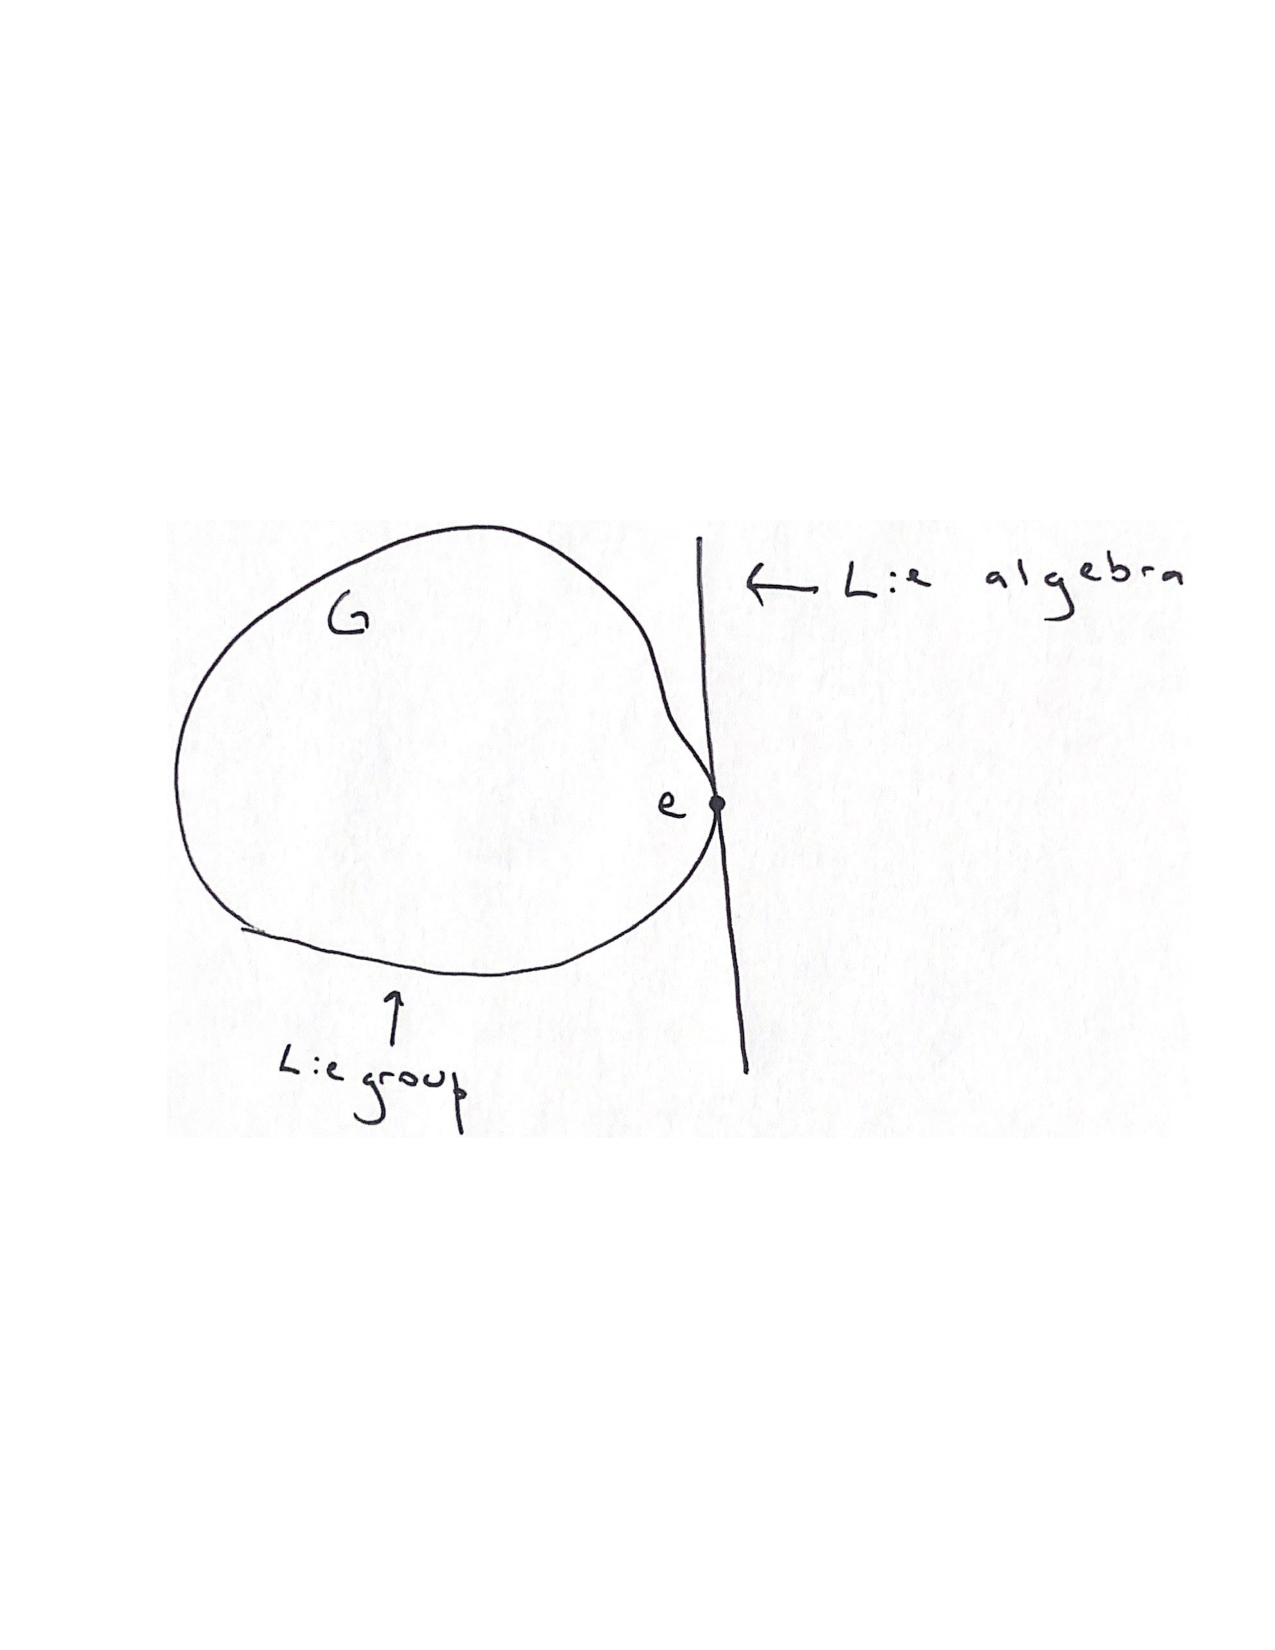
\includegraphics[scale=0.5]{images/tangentspace}
		\caption{The Lie algebra corresponding to a Lie group $G$ is the tangent space at the identity.}
	\end{center}
\end{figure}

A  \defn{first-order differential operator}\index{first-order differential operator} is a sum
\begin{align*}
	\sum_{i=1}^{d} f_{i}(X_1,\hdots,X_{d}) \frac{\partial}{\partial X_{i}}.
\end{align*}
First-order differential operators are, more or less, the same as vector fields on a manifold.
One can think of a vector field on a manifold as an infinitesimal automorphism that pushes each point an ``infinitesimal'' distance along the vector at that point.

Let $D = \sum_{i=1}^{d} f_{i}(X_1,\hdots,X_{d})\partial/\partial X_{i}$ and $E = \sum_{i=1}^{d} g_{i}(X_1,\hdots,X_{d})\partial/\partial X_{i}$ be first-order differential operators.
One can write
\begin{align*}
	D E &= \sum_{1\le i,j\le d}^{} f_{i} \frac{\partial}{\partial X_{i}} g_{j}\frac{\partial}{\partial X_{j}}\\
		 &= \sum_{1\le i,j\le d}^{} f_{i}g_{j}\frac{\partial}{\partial X_{i}}\frac{\partial}{\partial X_{j}} + f_{i}\frac{\partial g_{j}}{\partial X_{i}}\frac{\partial}{\partial X_{j}}.
\end{align*}
Similarly,
\begin{align*}
	ED &= \sum_{1\le i,j\le d}^{} f_{i}g_{j}\frac{\partial}{\partial X_{i}}\frac{\partial}{\partial X_{j}} + g_{j}\frac{\partial f_{i}}{\partial X_{j}} \frac{\partial}{\partial X_{i}}.
\end{align*}
Though $DE$ and $ED$ are not first-order, $DE-ED$ is first-order.
One can defines the \defn{Lie bracket}\index{Lie bracket} to be
\begin{align*}
	[D,E] := DE - ED.
\end{align*}

\begin{exercise}\label{}\text{}
Suppose that $D$ and $E$ are differential operators of orders $m$ and $n$ respectively.
Show that $[D,E]$ has order $m+n-1$.
\end{exercise}

One can see that 
\begin{align*}
	[D,E] = -[E,D].
\end{align*}
There is also the \defn{Jacobi identity}\index{Jacobi identity}:
\begin{align*}
	[[A,B],C] + [[B,C],A] + [[C,A],B] = 0.
\end{align*}
This is true for any (associative) ring.

\begin{definition}[ ]\label{}\text{}
A \defn{Lie algebra}\index{Lie algebra} $\mathfrak{g}$ is a vector space over $\mathbf{R}$ or $\mathbf{C}$ that has a bilinear map 
\begin{tikzcd}[cramped]
	{[}\ ,\ {]} : \mathfrak{g}\times \mathfrak{g}\ar[r]& \mathfrak{g}
\end{tikzcd}
that satisfies 
\begin{align*}
	[x,y] =- [y,x]
\end{align*}
and
\begin{align*}
	[[x,y],z] + [[y,z],x] + [[z,x],y] =0
\end{align*}
for all $x,y,z\in \mathfrak{g}$.
\end{definition}

\begin{remark}
	One can take $\mathfrak{g}$ to be a module over a commutative ring.
\end{remark}

Let $G$ be a Lie group with identity $e$. Let $T_{e}G$ be the tangent space to $G$ at $e$.
Notice that $G$ acts on itself by left translation. A left-invariant vector field on $G$ is uniquely determined by its value at $e$. That is, left-invariant vector fields on $G$correspond to tangent vectors to $G$ at $e$.
Vector fields correspond to first-order differential operators, so the left-invariant vector fields on $G$ are closed under the Lie bracket. Left-invariant vector fields correspond to tangent vectors to $G$ at $e$, so $T_{e}G$ has a Lie bracket. Thus, we define the Lie algebra of a Lie group $G$ to be 
\begin{align*}
	\mathfrak{g} := T_{e}G.
\end{align*}

\begin{example}[ ]\label{}\text{}
Consider $G =\mathbf{R}^{n}$ with addition.
The left-invariant vector fields on $G$ are of the form
\begin{align*}
	\sum_{i=1}^{n} a_{i} \frac{\partial}{\partial X_{i}}
\end{align*}
where $a_{i}$ is constant.
The Lie bracket of any two such operators is $0$, so the Lie algebra of $G$ is commutative. 
\end{example}

\iffalse
\begin{example}[ ]\label{}\text{}
Let $\mathfrak{g}$ be the Lie algebra of $G = \GL_{n}(\mathbf{R})$. The identity of $G$ is the identity matrix $e$, and the tangent space to $G$ at $e$ can be identified with $M_{n}(\mathbf{R})$.
Let $x\in M_{n}(\mathbf{R})$. What does the vector field $D$ corresponding to $x$ look like?
For a function $f$ on $\GL_{n}(\mathbf{R})$, this vector field is given by
\begin{align*}
	Df = \frac{f(a(1+\eps x)) - f(a)}{\eps}
\end{align*}
for $a\in G$.
This is the lowest order term of $f(a (1+\eps x)) - f(a)$, which is $\eps$ times something, which we want, plus higher order terms.

Let $x$ and $y$ be vector fields corresponding to differential operators $D$ and $E$ respectively.
Then, at $a\in G$, $(ED)f$ is the lowest order term of
\begin{align*}
	f(a(1+\delta y) (1+\eps x)) - f(a(1+\delta y)) - f(a(1+\eps x)) + f(a),
\end{align*}
which is $\eps\delta$ times something, which we want, plus higher order terms.
One sees that $(DE)f$ is similar and $(DE-ED)f$ is the lowest order term of 
\begin{align*}
	f(a(1+\eps x) (1+\delta y)) - f(a(1+\delta y) (1+\eps x)).
\end{align*}
Taking $a$ to $(1+\eps x-\delta y + \delta \eps yx)a$, this is the lowest order term of
\begin{align*}
	f(a(1-\delta\eps yx + \eps\delta xy)) - f(a),
\end{align*}
which is the differential operator corresponding to $xy-yx$. Thus, the Lie bracket of differentiable operators corresponding to matrices $x$ and $y$ is $xy-yx$, so we get the same bracket whether we consider $x$ and $y$ as matrices or left-invariant vector fields.  

It follows that the Lie algebra of $G$ is $\mathfrak{g} = M_{n}(\mathbf{R})$ with Lie bracket $[x,y] = xy-yx$.
For a closed subgroup of $\GL_{n}(\mathbf{R})$, the tangent space at $e$ is a subspace of $M_{n}(\mathbf{R})$ and the Lie bracket one gets is the restriction of the one above.
\end{example}

\begin{example}[ ]\label{}\text{}
Consider $G=\SL_{n}(\mathbf{R})$. Then, the tangent space $T_{e}G$ consists of matrices $x$ such that $\det(1+\eps x) = 1 + O (\eps^{2}) = 1 + \eps \tr(x) + \eps ^{2}\cdots$, so $\tr(x)=0$.
Thus, the Lie algebra of $\SL_{n}(\mathbf{R})$ is $n\times n$ matrices with trace $0$.
\end{example}

\begin{example}[ ]\label{}\text{}
Consider $G = O_{n}(\mathbf{R}) = \{x\in M_{n}(\mathbf{R}) : xx^{*}=e\}$. 
The tangent space $T_{e}G$ consists of matrices $x$ such that $(e+\eps x)(e+\eps x) ^{*}=  e + O(\eps^{2})$.
Since $(e+\eps x) (e+\eps x) ^{*} = e + \eps x + \eps x ^{*} + \eps ^{2}xx^{*}$, $T_{e}G$ (that is, the Lie algebra) consists of matrices with $x+x^{*}=0$.
\end{example}

One can compute the Lie algebra differently.
For example, let $G=\GL_{n}(\mathbf{R})$.
One defines $[x,y]$ to be the lowest-order term of the commutator $a^{-1}b^{-1}ab$ where $a\approx 1+\eps x$ and $b\approx 1+\delta y$ are elements of $G$ and $x$ and $y$ are tangent vectors. 
One sees that
\begin{align*}
	a^{-1}b^{-1}ab &= (1-\eps x) (1-\delta y)  (1+\eps x) (1+\delta y)\\
		       &= \eps\delta (xy-yx) + \textrm{higher order terms.}
\end{align*}
One gets the Jacobi identity here from the \defn{Hall--Witt identity}\index{Hall--Witt identity}:
\begin{align*}
	[[x,y^{-1}],z]^{y}[[y,z^{-1}],x]^{z}[[z,x^{-1}],y]^{x} = 1
\end{align*}
where $[x,y] = x^{-1}y^{-1}xy$ and $x^{y}=y^{-1}xy$.
\fi


\iffalse
\section {Lie groups and Lie algebras}

\section {The exponential map}

\section {The Poincar\'e--Birkhoff--Witt theorem}

\section {The Baker--Campbell--Hausdorff formula}

\section {Positive characteristic is weird}

\section {Bianchi classification}

\section {Engel's theorem}

\section {Lie's theorem}

\section {The Haar measure}
\fi

\printindex

\end {document}
